\documentclass[12pt]{article}
\usepackage{amsmath}

\title{GPU optimization of base form 820 - collective artificial spouse retirement plan}
\author{Nikolaj Aaes, Niklas Schalck Johansson and Hildur Uffe Flemberg}
\date{22-05-2013}

\begin{document}
	\maketitle
	
	% noter:
	% Command + >/< skifter mellem PDF og .txt i textmate \\
	% http://www.stdout.org/~winston/latex/latexsheet.pdf er et cheatsheet for \LaTeX{}
	
	\section{Abstract}
	
	%!TEX root = /Users/Nikolaj/Developer/GPU-Project/Report/Report.tex
%Abstract is the executive summary of the entire paper. As a summary it should encompass not only the main result, but also the problem, and the evaluation. Shaw [4] reports that good ICSE papers discussed evaluation already in their abstract. This is important in software engineering, because of the emphasis put on the evaluation of results.
%A good abstract is readable for non-experts, as it increases the chances that someone will build on your work (often application opportunities appear in other areas).
%I try to have four sentences in my abstract. The first states the problem. The second states why the problem is a problem. The third is my startling sentence. The fourth states the implication of my startling sentence.

%Simon Peyton Jones summarizes this idea in the following points

%Statetheproblem
%Saywhyit’saninterestingproblem 
%Saywhatyoursolutionachieves
%Saywhatfollowsfromyoursolution

This paper explores how utilizing CUDA C and general purpose graphic processing units can make the calculation of reserves for the Base Form 820 Collective Artificial Spouse Retirement Plan, faster. \\

In its current state this calculation take more than 20 minutes per customer if a decent approximation of the reserve is to be achieved. The parallelized solution presented in this paper makes it up to INDSÆT TAL times faster than the original solution, meaning that the previous 20 minute execution now takes INDSÆT TAL seconds. \\

The solution enables insurance companies to estimate the reserves for Base Form 820 using relatively cheap hardware, much faster than previously.

	
	\section{Introduction}
	
	This report is written at the IT University of Copenhagen (ITU) in the spring term of 2013 in connection with a CUDA project supervised by Peter Sestoft from ITU and Hans Henrik Brandenborg Sørensen from the Technical University of Denmark (DTU). The report is addressed to people interested in exploiting the benefits of using general purpose graphical processing units (GPGPUs)\footnote{Graphical Processing Units (GPUs) are most commonly used to render graphics in computer games. GPGPUs are ``general purpose'' variants that share the same architecture as GPUs but are optimized for computing purposes out of line with the graphics category. Since this project is not about graphics, we will refer to GPGPUs simply as GPUs, for shortness, throughout the rest of the report.} to optimize feasible computations in general, but specifically to people interested in CUDA.\\

In this project, we take a problem from the insurance industry that requires a significant amount of time to solve and show how to speed it up using the GPU. The problem concerns life insurance policies for married people, where one of them receives an amount of money some time after the other person has died. The goal, from the view of the insurance company, is to estimate its holding as accurately as possible to always be able to satisfy the obligation to the policyholder. Such an estimate is largely dependent on a guess of when the policyholder is going to die which can be anytime between signing of the policy and some, possibly large, number of years ahead in time. Furthermore, the time of death is dependent on several variables like age, gender etc. \\

The insurance company has a mathematical model that unifies all these variables and can be solved by a computer but it takes a lot of time to do - even with modern CPUs. Moreover, insurance companies typically issue several thousands of policies, each of which has an impact on the complexity of the computation as well as the size of the overall reserves the company needs to hold back in case a disbursement is claimed. All these facts together make computing power a valuable entity. The goal of this project is to analyze the opportunity to speed up the computation for a single policyholder through parallelism with CUDA, i.e. to optimize the time it takes to compute the size of the reserves needed at any time during the life of a policyholder such that the insurance company can fulfill its obligations when the person dies.\\

The reader of the report is assumed to know the basic principles of concurrency and parallelism. No CUDA specific knowledge is required.
		
	\section{Background}
	SCOPE: Vi kører kun med een kunde ikke flere
		
	%!TEX root = /Users/Nikolaj/Developer/GPU-Project/Report/Report.tex

TODO
%- Related work, projects that precedes this project, why do we use the technology described, what is this new technology
%- Nævn at vi har fået udleveret matematik beforehand

\subsection{Problem definition}
How can CUDA C be utilized to optimize the calculation of the baseform 820 collective artificial spouse retirement plan using the Runge Kutta 4th order method?

\subsection{Scope}
	The scope of this project is to handle a single customer at a time. We do not explore the possibilities for optimizing the process of using the algorithm on several customers at a time. Neither do we explore alternative methods for approximating differential equations.
	
\subsection{Assumptions}
This project was developed under several assumptions to limit the size of it. We assumed that the spouse of an insurance holder was always of the opposite gender. It would now be possible to take same-gender couples into account but it would require som modification to the code. We assumed that the function to determine the interest rate always returns 5 \%. 



		
	\section{The Math}
		
	%!TEX root = /Users/Nikolaj/Developer/GPU-Project/Report/Report.tex
%- Description of the insurance math used in the current solution \\
\label{themath}
The content of this section is defined by the mathematical specification\cite{edlu} provided by the insurance company. The algorithm in this project is used to determine the reserve the insurance company needs to possess to be able to pay the insurance holder's spouse in the case of his or her death. We assume that the spouse of the insurance holder is of the opposite gender. If the insurance holder does not have a spouse at the time of his or her death the insurance is forfeited. \\

The algorithm used is a 4th order Runge-Kutta solver with a fixed stepsize (indsæt reference) where we use a series of constants determined before any calculation begins:

\begin{table}
\begin{center}
\begin{tabular}[t]{|c|c|}
	\hline
\textbf{Name}&\textbf{Meaning}\\\hline
$\tau$&The time of death of the insurance holder\\\hline
$r$&The pension age\\\hline
$g$&The grace period\\\hline
$x$&The age of the insurance holder at calculation time ($t$ = 0)\\\hline
$t$&The time of calculation\\\hline
$h$&The Stepsize of the Runge-Kutta solution\\\hline
\end{tabular}
\end{center}
\caption{Constants}
\label{table:constants}
\end{table}

$\tau$ is expressed as $x+t$. Apart from this there is also a constant $k$ which is determined by $\tau, r$ and $g$ in the following manner:

\begin{table}
\begin{center}
	\begin{tabular}[t]{|c|c|}
		\hline
		\textbf{If this statement holds}&\textbf{then $k$ equals}\\\hline
		$\tau < r$&$g$\\\hline
		$r \leq \tau < r + g$& $r + g - \tau$\\\hline
		$r + g \leq \tau$&0\\\hline
	\end{tabular}
\end{center}
\caption{How $k$ is defined}
\end{table}

The algorithm can be described as a combination of three models; an outer model that describes the life/death state of the insurance holder, a middle model that describes the married/unmarried state of the insurance holder and an inner model that describes the life/death state of the potential spouse. \\

NOTE: The description in the three model sections is loosely based on a description for Edlund\cite{edlu} and some passages are directly translated from this document.

\subsection{Outer Model}
The outer model is expressed as the following equation:
\begin{equation}
\frac{d}{dt} f(t) = r(t) f(t) - \mu_t(x+t) (S_{x+t}^d (t) - f(t)) 
\end{equation}

Where $S_\tau^d$is the death benefit that for a $\tau$ year old at the time $t$ is needed to cover the payment from the insurance company, $\mu_t(x+t)$ is the mortality rate for a $(x + t)$ year old and $r(t)$ is the interest rate function. In this project the interest rate function returns the constant 0.05.

The differential equation is solved from $t=120-x$ to $t=0$ with the boundary condition $f(120-x)=0$.

\subsection{Middle Model}
The middle model is used to calculate $S_{x+t}^d (t)$ and is expressed with the following equation: 

\begin{equation}
S_\tau^d(t) = \left\{ 
  \begin{array}{l l}
    	g_\tau \int	f(\eta|\tau)a_{[\eta] + g}^I(t)d\eta									& \quad \text{$\tau \le r$}\\
    	g_\tau \int	f(\eta|\tau)a_{[\eta] + r + g - \tau}^I(t)d\eta 			& \quad \text{$r \leq \tau \le r + g$}\\
			g_\tau \int	f(\eta|\tau)a_{[\eta]}^I(t)d\eta 											& \quad \text{$r +g \leq \tau$}
  \end{array} \right.
\end{equation} \\

Where $g_\tau$ is the probability that a $\tau$ year is married and $f(\eta|\tau)$ is the probability distribution for, that a $\tau$ year old is married to a $\eta$ year provided that the $\tau$ year old is married.
This equation can be rewritten to this form: 

\begin{equation}
\frac{d}{dn}f(\eta) = -g_\tau f(\eta|\tau)a_{[\eta]+k}^I(t)
\end{equation}

here the subscript for $a$ is rewritten to $[\eta]+k$ where $k$ can fall into three different categories as shown in table \ref{table:constants}. 

This differential equation is solved from $\eta = 120$ to $\eta = 1$ with the boundary condition $f(120) = 0$.

\subsection{Inner Model}
The inner model is used to calculate $a_{[\eta]+k}^I(t)$ and is expressed with the following equation:

\begin{equation}
\frac{d}{ds}f(s) = r(t+s)f(s) - 1_{s \geq k} - \mu_{t+s}(\eta + s)(0 - f(s))
\end{equation}

Where $t$, $\eta$ and $k$ are constants and $\mu_{t+s}(\eta + s)$ is the mortality rate for a $(\eta + s)$ year old.

This differential equation is solved from $s = 120 - \eta$ to $s = 0$ with the boundary condition $f(120 - \eta) = 0$

\subsection{Runge-Kutta 4th order}
The Runge-Kutta method is a method for numerically solving differential equations that builds on Eulers method \cite{nric} and the midpoint method \cite{nric}. When given a start point and a differential equation one can choose a stepsize and approximate the graph.
When given a point $(x_n,y_n)$, a differential equation $f$ and a stepsize $h$ one can use the Runge-Kutta method to approximate the next point in the following way:

\begin{align}
\nonumber &k1 = h f(x_n, y_n) \\
\nonumber &k2 = h f(x_n + \frac{h}{2}, y_n + \frac{k1}{h} ) \\
\nonumber &k3 = h f(x_n + \frac{h}{2}, y_n + \frac{k2}{h} ) \\
&k4 = h f(x_n + h, y_n + k3 )
\end{align} 

\begin{align}
\nonumber& x_{n + 1} = x_n + h \\
&y_{n + 1} = y_n + \frac{k1}{6} + \frac{k2}{3} + \frac{k3}{3} + \frac{k4}{6} + O(h^5)
\end{align}

The component $O(h^5)$ denotes the error per step and is sufficiently small to be ignored in this project.

\subsection{Description of Execution}
	To provide a better overview of how the mathematical principles are applied we go through how an execution is performed. Before the execution begins certain value are give before hand, namely $g$, $r$ and $x$. Additionally we need to decide on a stepsize before the execution can begin. \\
	
	The first step in the execution is to use the outer model with a starting point. Since the outer model is to be solved for $t=120-x$ to $t=0$ with the boundary condition $f(120-x)=0$ we can use the point $(120-x, 0)$ as our starting point. The next step is to actually solve the outer model equation to calculate the next approximate point. All the components in the outer models differential equation can be computed using normal equations except $S_{x+t}^d (t)$. This component can be calculated using the middle model and when it computed the calculation of the next approximate point is completed. The outer model equation is solved four times for each approximation of the next point corresponding to calculating $k1$, $k2$, $k3$ and $k4$ in the Runge Kutta method. This can be repeated $(120-x) \times stepsize$ times until the approximate point becomes $(0,y)$ which is the final point. \\
	
	To calculate the missing component using the middle model we need to establish the value of $k$ for the point. Additionally we are given the value $t$ from the outer model. Like the outer model we need to use the middle model with a starting point. The middle model is to be solved for $\eta = 120$ to $\eta = 1$ with the boundary condition $f(120) = 0$ which means that we can use $(120,0)$ as our starting point. As with the outer model all the components of the differential equation in the middle model can be computed using normal equations except $a_{[\eta]+k}^I(t)$. This can be calculated using the inner model which is the last model in the chain. When the inner model has computed a result the calculation of the next approximate point is completed. As in the previous model the middle model equation is calculated four times corresponding to calculating $k1$, $k2$, $k3$ and $k4$ in the Runge Kutta method. This can be repeated $119 \times stepsize$ times until the approximate point becomes $(0,y)$ which is the final point and the $y$-value of this point is returned to the outer model. \\
	
	As the last part of the execution the inner model needs to calculate the last component used by the middle model. The inner model uses the $t$, $k$ and $\eta$ values provided by the middle model. This model uses a starting point in the same way as the other models. This model is to be solved for $s = 120 - \eta$ to $s=0$ with the boundary condition $f(120 - \eta) = 0$ which means we can use the point $(120-\eta,0)$ as a starting point. Contrary to the other two models the inner model equation only contain components that can be computed using normal equations to find the next approximate point. For each approximation of a point the inner model equation is solved four times corresponding to calculating $k1$, $k2$, $k3$ and $k4$ in the Runge Kutta method. This can be repeated $(120 - \eta) \times stepsize$ times until the approximate point becomes $(0,y)$ which is the final point and the $y$-value of this point is returned to the middle model. \\ 
	
	In any execution the outer model equation will be solved 
	
	\begin{equation}
	(120-x) \times stepsize \times 4
	\end{equation} times, the middle model equation will be solved 
	
	\begin{equation}
	((120-x) \times stepsize) \times (119 \times stepsize \times 4)
	\end{equation} times, and the inner model equation will be solved 
	
	\begin{align}
 \nonumber&((120-x) \times stepsize \times 4) \times  
	(\sum\limits_{i=120 \times stepsize}^{stepsize+1} 
	( 
	(120 - \frac{\eta}{stepsize}) \times stepsize \times 4) \\ \nonumber & + 
	((120 - \frac{2\eta - 1}{2 \times stepsize})\times stepsize \times 4) + 
	((120 - \frac{2\eta - 1}{2 \times stepsize})\times stepsize \times 4) \\& +
	(120 - \frac{\eta-1}{stepsize}) \times stepsize \times 4)
	)
	\end{align} times.\\
	
	For a normal execution with $stepsize=4$, $g=30$, $r=80$ and $x=115$ the outer model equation will be solved 80 times, the middle model equation will be solved 152.320 times and the inner model equation is solved 145.008.640 times.

	
	BESKRIV HVORDAN EN NORMAL KØRSEL SERUD = EKSEMPEL
	kig evt på en simpson integration når vi kigger på middle da det egentlig ikke er en differential ligning men et integrale
		
	\section{CUDA}
en tråd skal lave et vist stykke arbejde før det kan betale sig at oprette den. Der er overhead for at lave context for hver tråd så hvis den arbejde tråden laver er mindre end at sætte overheaden op, giver det ingen mening.

	%!TEX root = /Users/Nikolaj/Developer/GPU-Project/Report/Report.tex
		- A more elaborate description of GPGPUs, architecture and CUDA C.
		
		\subsection{Parralellisation}

De forskellige parallelliserings muligheder:
- beskriv teorien
- beskriv hvad vi får ud af det i køretid?
- beskriv hvorfor vi har/ikke har valgt denne løsning
- Kan den kombineres med de andre for bedre performance?\\

Outer Par \\
Da man på forhånd kan beregne alle x værdier outer skal bruge i sin kørsel og alle Middle(x) kald i outerDiff kun skal bruge en x værdi er det muligt at regne alle disse middle kald i parallel og gemme hvert middle kalds resultat i et array. Når man derefter skal gå fra startpunkt til næste punkt kan man betragte Middle(p.x) i $return r_(px) * py - GmFemale(x + px) * (Middle(px).y - py);$ som en udregning der tager konstant tid.\\

Middle Par\\
Da man på forhånd kan beregne alle x værdier middle skal bruge i sin kørsel og vi ved at hvert step i Middle har udregninger til k1,k2/k3 og k4 i hvert skridt der kun afhænger af x-værdien kan vi regne alle de sæt af k1,k2/k3 og k4 som middle skal bruge i parallel. Derefter kan de lægges sammen som et vægtet gennemsnit i et array og bruger når man vil gå fra et punkt til et nyt. Kaldet $double y = p.y + k1/6 + k2/3 + k3/3 + k4/6;$ kan altså betragtes som konstant. Her udregnes hvert sæt af k1, k2/k3 og k4 dog i en enkelt tråd. Det vil sige at der er een tråd for hvert step.\\

Inner Par\\
Man har også muligheden for at parallisere middles kald til inner der bruges i udregningen af k1, k2/k3 og k4. Ved at sætte 3 tråde til at udregne de tre værdier kan dette gå tre gange så hurtigt.\\

Kombination af Outer Par og Middle par\\
Ved en valgt block size b = antal outersteps og en thread per block tpb kan man sætte hver block til at tage sig af en x-værdi i outer, altså tage sig af et enkelt middle kald. Hvis man forestiller sig at middle skal tage ms steps og ms > tpb, vil man først udregne k1, k2/k3 og k4 sæt for de først tpb steps og derefter gå videre til de til næste tpb steps indtil alle steps er udregnet. Det betyder også at der kan være inaktive tråde i den sidste omgang tpb steps og det kan give divergence. Det er muligt at bruge reduction (se cuda bogen) når alle k er blevet regnet ud og man skal lægge p.y til.\\

Kombination af Middle par og Inner par\\
Ligesom i den ovenstående løsning lader man hver block handle en x-værdi for middle og giv hver block tre tråde hver af disse tråde udregner hver sin k værdi og hver tredje tråd lægger dem sammen.\\

Kombination af alle tre\\
Som i kombinationen af outer par og middle oar vælger man et antal blokke svarende til antallet af outersteps og en thread per block tpb. Man lader stadig hver blok tage sig af et enkelt kald til Middle med en bestemt x-værdi. Forskellen kommer når man i stedet for at lade hvert tråd udregne et sæt af k1, k2/k3 og k4 værdier sætter man i stedet 3 tråde til at udregne dem i parallel. Dette vil kun have indvirkning hvis block størrelsen er større end det antal steps middle skal udføre. Hvis ikke  bruger man tre gange så mange tråde til at så udregnes først tpb k-værdier, tre gange hurtigere end normal, dernæst de næste tpb k-værdier, stadig tre gange så hurtigt men i stedet for at stoppe ved middlesteps som normal vil man stoppe ved middlesteps*3 da der skal bruges 3 gange så mange k-værdier. Optimalt set skal der altså være middlesteps*3 tråde i hvert block. Ved en vilkårlig stepsize vil det være 120*stepsize*3 tråde. Med en stepsize på 1 eller to giver det hendholdsvis 360 og 720 tråde hvilket stadig er inden for det 1024-tråde limit hver block har. Men allerede ved stepsize 3 giver det 1080 tråde per block hvilket ikke er legalt.\\

Hvad har vi valgt\\
Vi har valgt Kombination af Outer Par og Middle Par for simpelheden.
Kombination af alle tre er ikke smart fordi det kun giver optimering når threads per block er middlesteps*3 eller over hvilket ikke er legalt med en stepsize over 2.
SKRIV NOGET OM HVORFOR VI HAR VALGT KOMBI AF OUTER OG MIDDLE I STEDET FOR MIDDLE OG INNER. HVORFOR ER DET MERE EFFEKTIVIT?
		
	\section{Implementation}
		
	%!TEX root = /Users/Nikolaj/Developer/GPU-Project/Report/Report.tex
%Husk at nævne at Middle stepsize er hardcoded til 2.
%Husk at skrive noget om first step der i princippet ikke er en del af matematikken \\
%Husk at nævne at vi i Middle har sat k3 = k2;
%Husk at nævne at det antal steps vi tager kan variere i forhold til matematikken fordi vi tager et "Helt" step hver gang vi laver et firstStep hvor det jo i virkeligheden er en brøkdel af et step. Det gør ikke noget for resultatet, men hvis man tæller steps i programmet vil det ikke give det rigtige antal.
%	I den kode der er nu er insurance holder kvinde og spouse mand ALTID
%Husk at nævne at vi i Middle har sat k3 = k2;

After we established the mathematical base we implemented a C solution. Instead of implementing the solution directly into CUDA C we chose to implement a C solution first to eliminate any bugs that were purely C specific. This also made it easier to debug since CUDA C program are generally harder to debug (INDSÆT REF?). The implementation is based on the provided C\# code and to conform to that, the middle model's stepsize is always 2 and the insurance holder is always a woman and the spouse is always a man. \\

The first step was to implement the utility methods used for calculating trivial equations and were mostly taken directly from the original C\# implementation. The methods in question are \texttt{gTau(double tau)}, \texttt{f(double eta, double tau)}, \texttt{k(double tau, double r, double g)}, \texttt{r\_(double t)}, \texttt{GmFemale(double t)} and \texttt{GmMale(double t)}. These are all used to calculate components in each of the different differential equations. \\

The second step was to create the programs entry point, the main method. This would be responsible for initializing the $g$, $r$ and $x$ variable as well as the stepsizes for each model. \\

The next step was to split implement the base for the three models. Each model have a main method (\texttt{Outer(..)}, \texttt{Middle(..)} and \texttt{Inner(..)}), a method used for the Runge Kutta method (\texttt{OuterRK(..)}, \texttt{MiddleRK(..)} and \texttt{InnerRK(..)}) and a method that only contains the differential equation for the models (\texttt{OuterDiff(..)}, \texttt{MiddleDiff(..)} and \texttt{InnerDiff(..)}). While creating a Runge Kutta method for each model seems excessive because it serves a the same function in each model it was necessary later on because CUDA C does not support function pointers on compute capabilities lower than 2.0. If the implementation was only meant for the C programming language a single Runge Kutta method that took a function pointer would have been sufficient. \\

Each of the models main methods are responsible for executing the corresponding Runge Kutta method the correct number of times. This is done by calculating exactly how many full steps it needs to perform by using the \texttt{floor(double x)} method. When using this method we get an integer representation of how many steps we need to take in that particular model but since we are flooring the amount of steps there might be a step remainder smaller than 1, that we need to consider. To take this into account we use what we refer to as the first step. Before each model starts to perform the full number of steps it calculates the remainder of the flooring and takes a step to counter it. 
This is not necessary for the middle model since the middle model's stepsize is hardcoded to 2 which means that there will never be a remainder. It also means that the amount of full steps the middle model takes is constant and is therefore calculated in the programs main method. \\

As an additional optimization we found that the equations for calculating $k2$ and $k3$ in \texttt{MiddleRK(..)} are identical and chose to just calculate this value once and the use it both places. 

	I den kode der er nu er insurance holder kvinde og spouse mand ALTID
	skriv noget om memory bound og compute bound i rapporten
		
	\section{Testing}
	test på forskellige maskiner
	hvis vi deler steps op i blocks af 32 tråde kan der i worst case scenario være en sidste block med 1 aktiv og 31 inaktive tråde.
	Lav en graf over rest trådene
		
	- A test to ensure that the new implementation produces the same output as the current implementation


lige nu er insurance holder altid en kvinde og spouse altid en mand \\
		
	\section{Benchmarks and Comparison}
		
	%!TEX root = /Users/Nikolaj/Developer/GPU-Project/Report/Report.tex

Now that it has been established that the solution produces satisfactory results it is time to examine the increase in speed that the solution provides. Four different performance tests were performed each one providing a different insight into how this solution was improved compared to original C\# implementation. The graphs depicted in this section are all from the Gpulab06 machine because the performance of this machine was the best. Full performance tests for all machines can be found in Appendix \ref{app:graphs}. Note that the number of steps taken per year in the middle model is 2 for all test.\\

\subsection{Variable $x$}

Each step in the outer model takes equally long time to complete. This is because the number of steps taken in the middle and the inner model is constant as long as $h$ is constant. 
The relationship between the number of steps to take in the outer model and the time it takes to solve it can therefore be expressed as a linear equation. 
The number of steps in the outer model is solved from $120-x$ to 0 the $x$-value is proportional with the number of steps. This means that the running time is also a linear equation proportional with $x$.

It is important to show that our solution is fast no matter what values are chosen. Changing $g$ and $r$ will have no performance effect and is therefore not included in the tests.

\begin{figure}[ht!]
\begin{center}
	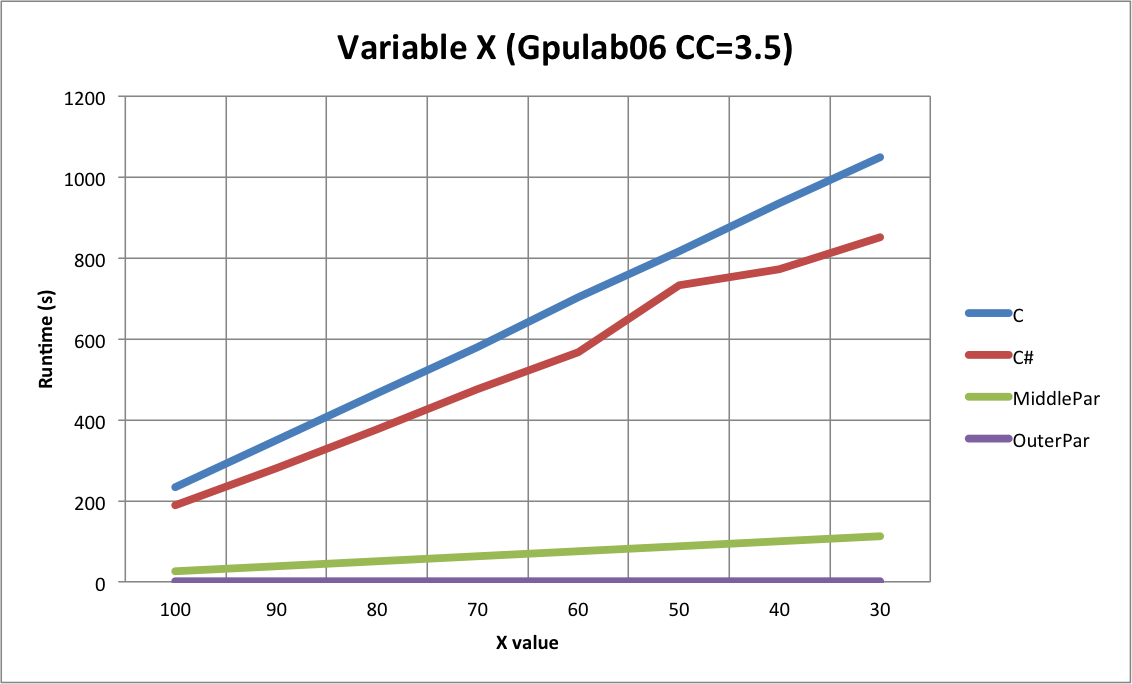
\includegraphics[width=\textwidth]{img/Gpulab-varx35.png}
\end{center}
\caption{The impact of changing the $x$ value on the Gpulab06 machine}
\label{variablex}
\end{figure}

When the $x$ value rises the runtime naturally increases because the outer model is solved from $120-x$ to 0. The lower the $x$ value the more steps needed. Our OuterPar solution is faster than the other implementations, and even though the runtime also increases for this solution it does not increase significantly. The results showed up to 665 times faster runtime compared to the original C\# solution.

\subsection{Variable Stepsize}
One of the advantages of using a 4th order Runge-Kutta solver is that an appropiate number of steps per year can be chosen to adjust the precision at the cost of an increase in running time. While increasing the steps per year will increase the running time in our implementation the increase is quite small compared to the C and C\# implementations.

\begin{figure}[ht!]
\begin{center}
	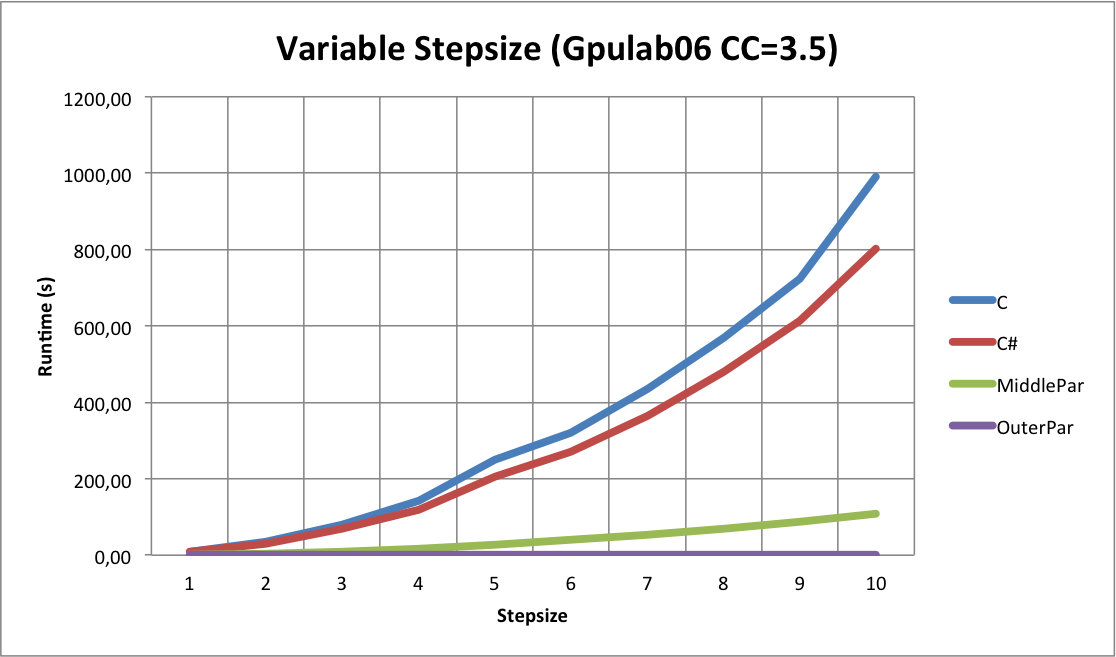
\includegraphics[width=\textwidth]{img/Gpulab-stepsize35.png}
\end{center}
\caption{The impact of changing the stepsize on the Gpulab06 machine}
\label{variablestepsize}
\end{figure}

Increasing the number of steps per year does increase the running time as expected but our OuterPar solution is superior in every test we performed on all the machines. The results showed up to 680 times faster running times compared to the original C\# implementation.

\subsection{Variable Threads per Block}
Since the number of threads per block is set at compile time in the CUDA implementations it is interesting to test what impact different amounts have on the performance.

\begin{figure}[ht!]
\begin{center}
	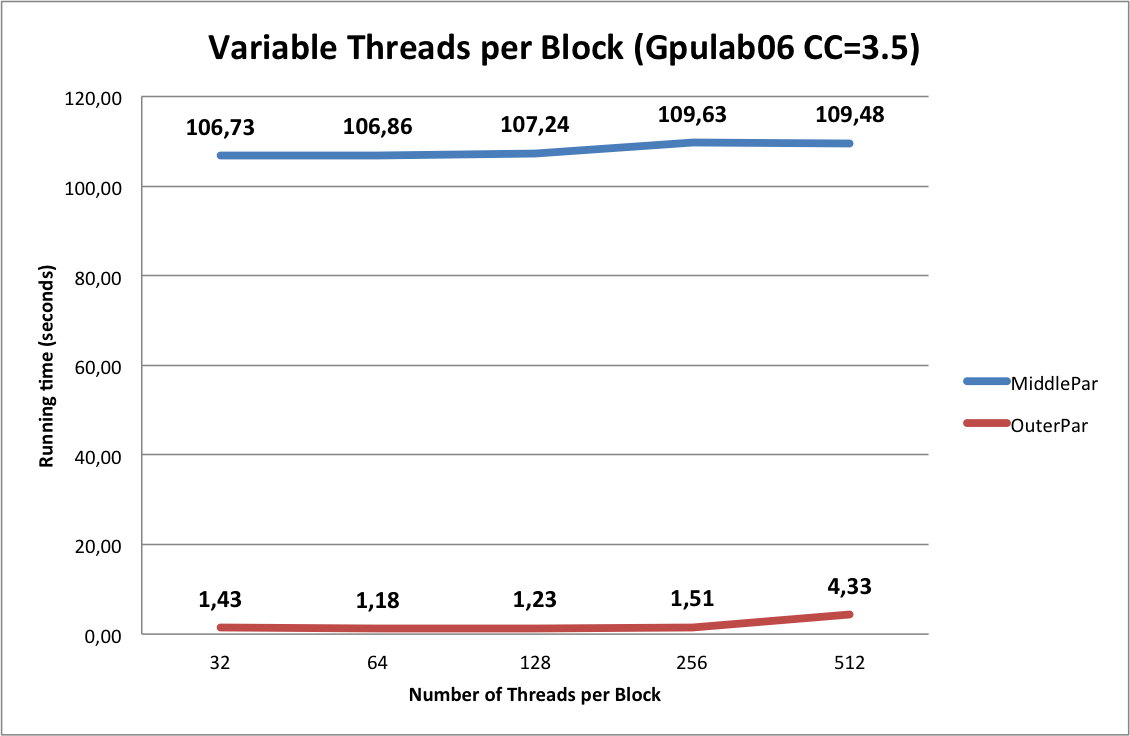
\includegraphics[width=\textwidth]{img/Gpulab-tpb35.png}
\end{center}
\caption{The impact of changing the threads per block on the Gpulab06 machine}
\label{ThreadsPerBlockGraph}
\end{figure}

\noindent As seen in Fig. \ref{ThreadsPerBlockGraph}, the slowest configuration is 512 threads per block. This is expected since the Gpulab06 GPU has a hardware limit of 2048 threads per SMP meaning that it schedules (2048 / 512) = 4 blocks at a time even though the hardware can schedule as many as 16. To increase performance, the amount of threads per block has to be lowered to yield more blocks and thus a better utilization of the SMPs. This fact explains the drastic improvement from 512 to 256 and from 256 til 128, at which the number of blocks reaches the exact hardware limit. Lowering the count further to 64 threads per block, however, seems to keep improving performance even though we already reached 16 blocks. \\

In this case, the explanation should be sought in the way SMPs divide threads of the executing blocks into warps. With a configuration of 64 threads per block, the SMP splits each block into 2 warps of 32 threads each instead of 4, 8 or 16 warps with 128, 256 and 512 threads per block respectively. The lower amount of warps that each block is split into, the fewer warps will have to leave the SMP when a single thread from a block is taking a long time to execute and cause the entire block to leave the SMP. This results in a faster exchange of blocks which means that the amount of threads in an SMP that is actually doing some work increases. \\

Using this line of thought, one could argue that having just 32 threads per block should be even faster. Considering the work that each thread is doing this is not the case. The middle model is solved from 119 to 1 yielding 238 steps in total with 2 steps per year. Since each step is taken care of by a thread, allocating more than 238 threads leaves som threads with no work to do while fewer than 238 require each thread to take more than one step. Looking at the graph, it is clear that the best balance between workload and number of threads lies somewhere between 32 and 64 threads per block on the Gpulab06 machine.

\subsection{Register Spilling}
It is worth mentioning that each kernel thread uses 68 registers which is more than the available limit on Nvidia GPUs with compute capability 3.0 or lower. Therefore, to reproduce these results, one should avoid register spilling by including -arg=sm\_35 when compiling the code with nvcc. In this way, the compiler will know that the code is going to run on GPUs with 255 registers available per thread. \\

The program will stop functioning if it is compiled with a compute capability between 2.0 and 3.0 and run with more than 512 threads per block because of the register limit. If it is run with less than 512 threads per block it will function but the runtime will be significantly reduced because of register spilling.

\subsection{Exp vs Pow}
After running all performance tests we discovered that the use of \texttt{exp} instead of \texttt{pow} in both the C and C\# implementation improved the running time substantially. Apparantly the \texttt{exp} function is much faster for calculation, and a few short tests showed an improvement i execution time between 20\% and 50\%. A future improvement should use \texttt{exp} instead of \texttt{pow}, as the change had no impact on the final reserve estimated by C and C\#.

\subsection{Results}
Looking at Fig. \ref{variablex} and Fig. \ref{variablestepsize} it is clear that they are not all perfectly linear even though it is mandated by the theory. The reason for this inconsistency is most likely that the implementations are run a computer whose resources are not allocated entirely for the program meaning that the amount of resources available for the program could vary during the execution. \\

From this section, we can conclude that both of the parallelized CUDA implementations are superior in running time compared to the C and C\# implementations. Furthermore, the running time of the OuterPar implementation surpassed the running time of the MiddlePar implementation in all tests performed.
		
	\section{Conclusion}
	
	Conclusion
	
	\section{Reflection / Discussion / Future improvements}
	improvements:
	det kan optimeres til at kunne køre flere kunder.
	Simpson løsning i middle?
	
	KUNNE DET VÆRE INTERESSANT AT BRUGE DYNAMIC PROGRAMMING?
	KUNNE MAN GEMME HVILKE KALD TIL INNER DER ER LAVET OG HVIS INNER SÅ KALDES IGEN MED SAMME VÆRDIER, KAN MAN SLIPPE FOR AT REGNE DET UD OG BARE HENTE RESULTATET. DOG SKAL MAN VÆRE OPMÆRKSOM PÅ AT MAN KAN KOMME I EN SITUATION HVOR EN BEREGNING SER AT DER IKKE ER NOGET RESULTAT FOR ET SÆT PARAMETRE OG DERFOR GÅR I GANG MED AT REGNE DET UD, MENS DEN FØRST BEREGNING KØRER KAN ANDRE BEREGNINGER MED SAMME PARAMETRE OG DE NYE BEREGNINGER VIL OGSÅ GERNE GEMME RESULTATET NÅR DE ER FÆRDIGE HVILKET KAN GIVE CONFLICTS (MÅSKE).
	eller
	Det kan være vi skal dokumentere en del om at man kan gemme alle resultater i en tabel og efter et vist antal kunder kan man ende med nok til bare at have opslag i stedet for beregninger. skal denne tabel et ligge på GPU så den kan slås op i konstant tid.
		
		skriv evt noget om autotuning, hvor programmet først tester med forskellige mængder af tråde og blokke og vælger den hurtigste løsning.
		
	%!TEX root = /Users/Nikolaj/Developer/GPU-Project/Report/Report.tex
%kig evt på en simpson integration når vi kigger på middle da det egentlig ikke er en differential ligning men et integrale
%simpson video: http://www.youtube.com/watch?v=ns3k-Lz7qWU

%kan det betale sig at køre dele af programmet på CPU'en?

%- Did we achieve what we wanted? what did we discover during the project? What can be changed in future implementations? \\

When computing reserves for several insurance holders one after another it could be beneficial to use tabulation and store the result of one or several models and the parameters they were given. Whenever a model is going to be solved with a specific input, the implementation could check if the result already exists and instantly return it instead of solving the model again. If the result was not found it could solve it and store the result for future use. \\ 

This approach is only beneficial when retrieving the result from storage is faster than solving the model. It is not beneficial if the amount of identical input parameters is too small. It would be interesting to examine the input parameter collision rate by solving the models for a large amount of insurance holders. The efficiency of this approach varies with the choice of data storage. \\

It could also be beneficial to have a mechanism for automatically determining the optimal amount of blocks and threads per block before running the kernel. An easy solution could be to implement an auto tuner that tests the running time with different amounts of blocks and threads per block and settles on the fastest. \\

If we examine Equation \ref{middlediff} used in the middle model it is a constant multiplied by an integral. This means that there is no need to use the Runge-Kutta method and we could have chosen another approach for integral approximating such as Simpson's rule \cite{simp}. Simpson's rule requires an even number of steps which our middle model will always have as long as the steps per year is an even integer. The Runge-Kutta method uses four calculations for each step ($k1$, $k2$, $k3$ and $k4$), whereas Simpson's rule only uses a single calculation. This could potentially make the estimation of the middle model four times faster but it also introduces the risk of reducing the precision in the result. In our implementation we have optimized the calculation of $k3$ as described in Section \ref{implementation} which means that Simpson's rule would only make the estimation of the middle model three times faster.

	Threats to validity???
	kan det betale sig at køre dele af programmet på CPU'en?
		
	\section{Glossary}
	
	\begin{itemize}
	\item Forsikringstager - insurance holder
	\item ægtefælle - Spouse
	\item livrente - life interest
	\item dødfaldssum
	\item pause periode - grace period
	\item randbetingelse
\end{itemize}
		
	\begin{thebibliography}{9}
			\bibitem{edlu} EDLUND DOKUMENTET
			\bibitem{pmpp} David B. Kirk, Wen-mei W. Hwu - Programming Massively Parallel Proccesors, A Hands-on Approach - Elsevier Inc. - 2010
	\end{thebibliography}
	
\end{document}